\documentclass{beamer}

\usepackage{helvet}
\usepackage{hyperref, graphicx}
\usepackage{amsthm}
\usepackage{etoolbox}
\usepackage{wrapfig}
\usepackage{tikz}
\usepackage{ulem}

\usetheme{default}
\setbeamertemplate{navigation symbols}{}
\AtBeginSection[ ]
{
\begin{frame}{Outline}
    \tableofcontents[currentsection]
\end{frame}
}

% Default fixed font does not support bold face
\DeclareFixedFont{\ttb}{T1}{txtt}{bx}{n}{11} % for bold
\DeclareFixedFont{\ttm}{T1}{txtt}{m}{n}{12}  % for normal - use in headings

% Custom colors
\usepackage{color}
\definecolor{TUGray}{RGB}{101,101,137}
\definecolor{TUBlack}{RGB}{30,0,0}
\definecolor{mygreen}{RGB}{45,111,63}
\definecolor{keywords}{RGB}{205,114,0}
\definecolor{comments}{RGB}{181,51,139}
\definecolor{strings}{RGB}{58,144,81}
\definecolor{numeric}{RGB}{66,110,176}
\definecolor{linos}{rgb}{0.4,0.4,0.4}
\definecolor{links}{rgb}{0,0.4,0.75}

\definecolor{bggray}{RGB}{232, 233, 235}

\usecolortheme[named=mygreen]{structure}
\setbeamercolor{normal text}{fg=TUBlack}\usebeamercolor*{normal text}

\setbeamercolor{codecol}{fg=TUGray!25!black,bg=bggray}

\hypersetup{colorlinks, linkcolor=links, urlcolor=links}

\usepackage[T1]{fontenc}
\usepackage[sfdefault,scaled=.85]{FiraSans}
\usepackage{mathpazo}


\usepackage{listings}

\newtoggle{InString}{}% Keep track of if we are within a string
\togglefalse{InString}% Assume not initally in string

\newcommand\digitstyle{\color{numeric}}
\makeatletter
\newcommand{\ProcessDigit}[1]
{%
  \ifnum\lst@mode=\lst@Pmode\relax%
   {\digitstyle #1}%
  \else
    #1%
  \fi
}
\makeatother

\lstset{literate=%
    {0}{{{\ProcessDigit{0}}}}1
    {1}{{{\ProcessDigit{1}}}}1
    {2}{{{\ProcessDigit{2}}}}1
    {3}{{{\ProcessDigit{3}}}}1
    {4}{{{\ProcessDigit{4}}}}1
    {5}{{{\ProcessDigit{5}}}}1
    {6}{{{\ProcessDigit{6}}}}1
    {7}{{{\ProcessDigit{7}}}}1
    {8}{{{\ProcessDigit{8}}}}1
    {9}{{{\ProcessDigit{9}}}}1
	{<=}{{\(\leq\)}}1
	{>=}{{\(\geq\)}}1,
	% morestring=[b]",
    % morestring=[b]',
    % morecomment=[l]{//},
}

\lstdefinelanguage{Pseudo}{
    morekeywords={return, while, if, for, input},
    morecomment=[l]{\#},
}

% Pseudocode style
\newcommand\pseudostyle{\lstset{
language=Pseudo,
basicstyle=\fontfamily{ccr}\scriptsize,
commentstyle=\it\scriptsize\color{linos},
keywordstyle=\it\bfseries\scriptsize,
mathescape=true,
literate=
    {=}{$\leftarrow{}$}{1}
    {==}{$={}$}{1}
    {<=}{{\(\leq\)}}1
	{>=}{{\(\geq\)}}1,
xleftmargin=18pt,
xrightmargin=4pt,
aboveskip=12pt,
belowskip=0pt,
frame=tB,
keepspaces=true
}}

% Python style for highlighting
\newcommand\pythonstyle{\lstset{
language=Python,
basicstyle=\ttfamily\tiny,
numbers=left,
numberstyle=\tiny\color{linos},
morekeywords={self, np},              % Add keywords here
keywordstyle=\tiny\color{keywords},
commentstyle=\it\tiny\color{comments},    % Custom highlighting style
stringstyle=\tiny\color{strings},
xleftmargin=18pt,
xrightmargin=4pt,
aboveskip=0pt,
belowskip=0pt,
escapeinside={(*@}{@*)},
frame=l,                         % Any extra options here
showstringspaces=false,
keepspaces=true
}}

% Pseudocode environment
\lstnewenvironment{pseudo}[1][]
{
    \pseudostyle
    \lstset{
        #1
    }
}
{}

% Python environment 
\lstnewenvironment{python}[1][]
{
	\pythonstyle
	\lstset{
	#1
	}
}
{}

% wrap the Python environment
\newenvironment{codeblock}
    {\hfill\begin{beamerboxesrounded}[lower=codecol, width=0.8\textwidth]
    \medskip

    }
    { 
    \end{beamerboxesrounded}\hfill
    }

\theoremstyle{example}
\newtheorem{question}{Question}

\newcommand{\ct}[1]{\lstinline[language=Python]!#1!}
\newcommand{\ttt}[1]{{\small\texttt{#1}}}
\newcommand{\lsitem}[2]{\ttt{{#1}[}\ct{#2}\ttt{]}}

\author{Chris Cornwell}
\date{Sept.~25, 2025}
\title{Numerical Optimization}

\begin{document}

\begin{frame}
\titlepage
\end{frame}

%%%%
\begin{frame}
\frametitle{General approach to numerical optimization}
    Approach to minimization of function $g$. 

    \pause
    \begin{enumerate}
        \item Start the process from some initial point ${\bf w}^{(0)}$.
        \pause
        \item After $t$ steps, with ${\bf w}^{(t)}$ as current input to $g$, update it to some ${\bf w}^{(t)}$, ``going downhill'' toward a stationary point. 
        \pause
        \item Repeat Step (2) {--} converging to a stationary point, in good scenario {--} until you meet a \textbf{stopping condition} at some step $T$. The approximate stationary point (potentially a minimizer) is ${\bf w}^{(T)}$.
    \end{enumerate}
    
    \centering 
    \includegraphics[]{}
\end{frame}

\section{Gradient Descent}

%%%%
\begin{frame}
\frametitle{The general procedure}
    Have a function $\mathcal L:\mathbb R^p \to \mathbb R$ (our case, a loss function with $\Omega=\mathbb R^p$). Want to approximate minimizer in $\mathbb R^p$ for $\mathcal L$. 

    \pause
    \begin{itemize}
        \item Select (any) initial $\omega^{(0)}\in \mathbb R^p$ and a learning rate $\eta_t > 0$ for each step $t\ge 1$.\footnote{In these slides, $\eta_t$ will be constant in $t$; however, in many scenarios $\eta_t$ decreases as $t$ increases.} 
        \pause
        \item Next, for $t\ge 1$, iteratively assign
        \[\omega^{(t)} = \omega^{(t-1)} - \eta_t\nabla\mathcal L(\omega^{(t-1)}).\]
        \pause
        \item Iterate until some \textbf{stopping condition} is met (say it happens when $t = T$). The approximate minimizer is $\omega^{(T)}$.
    \end{itemize}

    \pause
    More on stopping conditions later. For now, \ldots 
    \pause
    \begin{itemize}
        \item choose a (``small'') threshhold value $\varepsilon$. Stop when, as part of the last update, the \emph{change} in every parameter \emph{divided by its size} is not more than $\varepsilon$. \pause That is, stop when 
        {\small
        \[\frac{|\omega^{(t)}_j - \omega^{(t-1)}_j|}{|\omega^{(t-1)}_j|} \le \varepsilon,\qquad \forall 1\le j\le p.\]
        }
    \end{itemize}
\end{frame}

%%%%
\begin{frame}
    \frametitle{Batch, Mini-batch, and Stochastic Gradient Descent}
    In machine learning, our true interest is to minimize the \textit{population} loss function, meaning: \newline 
    \pause
    \begin{quote}
        Given our parameters $\omega\in\Omega$ and some point $({\bf x},y) \in \mathbb R^d\times Y$, we have a measure of loss for that point, $\mathcal L_{({\bf x},y)}(\omega)$ (``per-example'' loss); the population loss at $\omega$ is the \emph{expected value} of per-example loss, expectation with resp.~to $P_{X,Y}$.
    \end{quote}
    \pause
    Lacking access to population loss function, use empirical loss $\mathcal L_{\mathcal S}$, which gives expected value {--} mean {--} from $\mathcal S$ of per-example loss.

    \pause
    \textbf{Batch Gradient Descent:} gradient of $\mathcal L_{\mathcal S}$ is used in each update. 

    \pause
    \textbf{Stochastic Gradient Descent:} in each update, select one random point from $\mathcal S$ and use gradient of per-example loss at that point.

    \pause
    \textbf{Mini-batch Gradient Descent:} Between Batch and Stochastic. Each update, random subset $\mathcal S' \subset \mathcal S$ taken (fixed size); the gradient of $\mathcal L_{\mathcal S'}$ is used.

    \pause
    \emph{Important}: expected value of gradient used should be $\nabla\mathcal L_{\mathcal S}$ (which is, hopefully, close to gradient of population loss).
        
\end{frame}
    
%%%%
\begin{frame}
\frametitle{Example with Linear regression}
    % example of it working
    Last time: given sample data $\mathcal S$ for simple linear regression, and using MSE as empirical loss, $\mathcal L_{\mathcal S}(m,b) = \frac1n\sum_{i=1}^n(mx_i + b - y_i)^2$, we found 
        \[\nabla\mathcal L_{\mathcal S}(m,b) = 
        {\footnotesize
        \left( \frac{2}{n}\sum_{i=1}^n(mx_i + b - y_i)x_i, \quad \frac{2}{n}\sum_{i=1}^n(mx_i + b - y_i) \right).
        }
        \]
    
    \pause
    Example: batch gradient descent working on the \lstinline[language=Python, stringstyle=\ttfamily\color{strings}]{'Example1.csv'} data.

    \begin{wrapfigure}{R}{0.5\textwidth}
        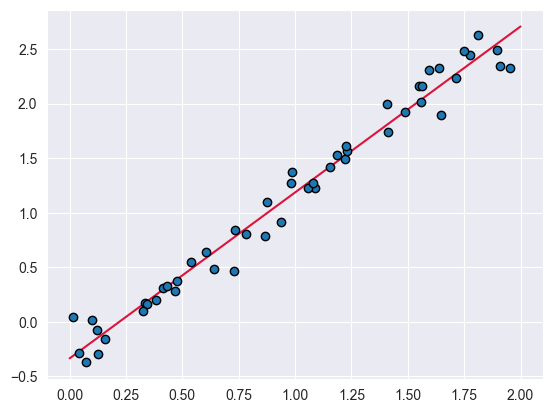
\includegraphics[width=0.47\textwidth]{../../Images/example1-lsrline.png}
    \end{wrapfigure}
    \phantom{line} \newline 
    \vfill
    The LSR line, using closed form. 
    \begin{itemize}
        \item $\hat{m}\approx 1.520, \hat{b}=-0.3346$:
    \end{itemize}
    \vspace{48pt}
    \vfill
\end{frame}

%%%%
\begin{frame}
    \frametitle{Example with Linear regression}
    % example of it working
    Last time: given sample data $\mathcal S$ for simple linear regression, and using MSE as empirical loss, $\mathcal L_{\mathcal S}(m,b) = \frac1n\sum_{i=1}^n(mx_i + b - y_i)^2$, we found 
        \[\nabla\mathcal L_{\mathcal S}(m,b) = 
        {\footnotesize
        \left( \frac{2}{n}\sum_{i=1}^n(mx_i + b - y_i)x_i, \quad \frac{2}{n}\sum_{i=1}^n(mx_i + b - y_i) \right).
        }
        \]
    
    Example: batch gradient descent working on the \lstinline[language=Python, stringstyle=\ttfamily\color{strings}]{'Example1.csv'} data.

    % ``seeing'' it converge
    \begin{wrapfigure}{R}{0.5\textwidth}
        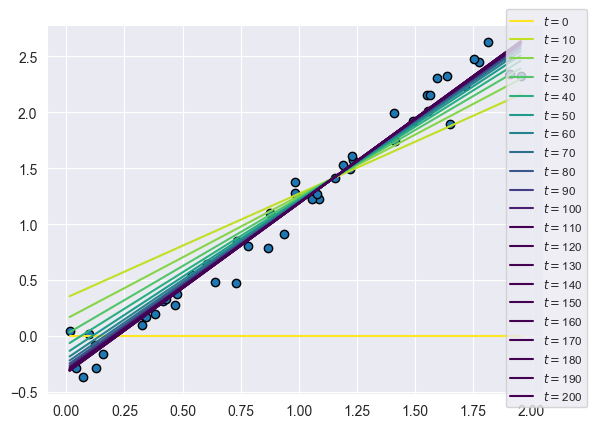
\includegraphics[width=0.47\textwidth]{../../Images/GDonExampleData.png}
    \end{wrapfigure} 
    \phantom{line}\newline 
    \vfill
    Plot of selected lines found during batch GD updates; starting parameters $m=0, b=0$; 
    
    \pause
    learning rate set to $0.1$.
    
    Parameter values on iteration 208: $m=1.519$, $b=-0.334$.
    \vfill
    
\end{frame}

%%%%
\begin{frame}[fragile]
    \frametitle{Implementing Gradient Descent}
    Some notes on implementation of the gradient descent updates.
    
    {\color{mygreen}1.} Each partial derivative of $\mathcal L_{\mathcal S}$, can compute it in one line of code. \pause Presuming \texttt{x} and \texttt{y} are arrays of coordinates for sample data, and that \lstinline[language=Python,basicstyle=\ttfamily,keywordstyle=\color{keywords}]{n = len(x)}, the following computes the partial derivatives:

\begin{codeblock}

\begin{python}
partial_m = (2/n)*np.sum( (m*x + b - y)*x )
partial_b = (2/n)*np.sum( (m*x + b - y) )
\end{python}

\end{codeblock}

    \pause
    {\color{mygreen}2.} To implement GD, want more than one function {--} at the least, one to compute the gradient (given current parameters); another that performs update and checks for stopping. \textit{Roughly}\ldots
\pause

\begin{pseudo}
## lr is learning rate; threshhold is for stopping;
input: X, y, lr, threshhold
p = initial array of parameters
while (max of last_update > threshhold){
    grad = compute_grad(p, X, y)
    last_update = | grad / p | ## entrywise array division
    # handle p[i] near 0
    p = p - lr*grad
}
return p
\end{pseudo}
\end{frame}

%%%%
\begin{frame}
    \frametitle{Convergence}
    Does gradient descent converge to point at which loss function is minimized? Is it even guaranteed to converge?

    \pause
    Short answer: No, not necessarily. 

    \ldots so, \textit{in what cases} can we guarantee such a thing?

    \phantom{To demonstrate the difficulty, imagine a ``toy'' loss function: $\ell:\mathbb R\to\mathbb R$ with $\ell(w) = w^2$. At each $w$ we have $\nabla\ell = \left(\frac{d\ell}{dw}\right) = (2w)$.} 

    \phantom{Say learning rate: $\eta > 1$. Then, at any $w^{(t)} > 0$, we get }
        \[\ \ \]
    \phantom{and so $|w^{(t+1)}| > |w^{(t)}|$. Likewise, if $w^{(t)} < 0$ then $|w^{(t+1)}| > |w^{(t)}|$.}
    
    \centering
    \begin{tikzpicture}
        \draw[opacity=0] (0,1) -- (0,0);
    \end{tikzpicture}
\end{frame}

%%%%
\begin{frame}
    \frametitle{Issues with convergence}
    To demonstrate the difficulty, imagine a ``toy'' loss function: $\ell:\mathbb R\to\mathbb R$ with $\ell(w) = w^2$. At each $w$ we have $\nabla\ell = \left(\frac{d\ell}{dw}\right) = (2w)$. 

    \pause
    Say learning rate: $\eta > 1$. Then, at any $w^{(t)} > 0$, we get 
        \[w^{(t+1)} = w^{(t)} - 2\eta w^{(t)} < w^{(t)} - 2w^{(t)} = -w^{(t)},\]
    and so $|w^{(t+1)}| > |w^{(t)}|$. \pause Likewise, if $w^{(t)} < 0$ then $|w^{(t+1)}| > |w^{(t)}|$.
    
    \pause
    So, it diverges when $\eta > 1$. However, if $0< \eta < 1$, then it will converge (to minimizer $w=0$).

    \pause
    \begin{figure}
    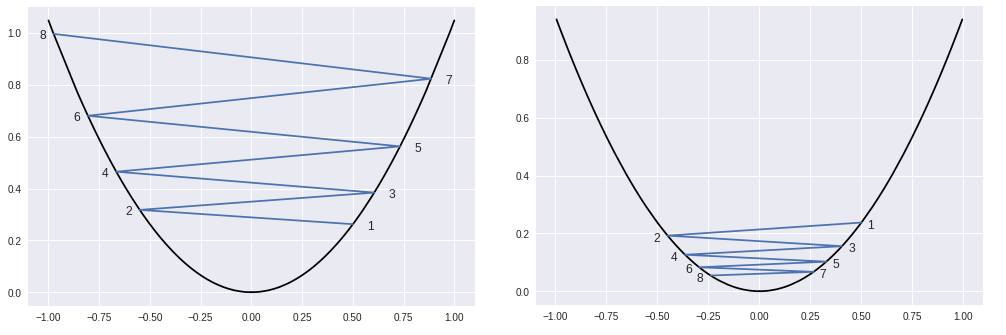
\includegraphics[height=0.3\textheight]{../../Images/GD-choosing-lr.png}
    \caption{Gradient descent on $\ell(w) = w^2$. Left: $\eta = 1.05$; right: $\eta = 0.95$.}
    \end{figure}
\end{frame}

%%%%
\begin{frame}
    \frametitle{Guarantees of convergence}
    If your loss function is differentiable and a \textbf{convex function}, and if have some ``control'' on size of the gradient then, by choosing $\eta$ small enough, can guarantee convergence. 

    \pause
    \begin{theorem}Suppose that $\mathcal L:\mathbb R^p\to\mathbb R$ is differentiable and convex, and suppose that $\nabla \mathcal L$ is \textit{Lipschitz continuous}\footnote{Meaning: $\exists$ a constant $C$ s.t.\ for all $\omega_1, \omega_2$, $|\nabla\mathcal L(\omega_1) - \nabla\mathcal L(\omega_2)| \le C|\omega_1 - \omega_2|$.} with some constant $C>0$ and that $\eta \le 1/C$. Then, for a minimizer $\omega^*$ of $\mathcal L$, 
            \[\mathcal L(\omega^{(t)}) - \mathcal L(\omega^*) \le \frac{|\omega^{(0)} - \omega^*|^2}{2\eta t}.\]
    \end{theorem}
    \pause
    \begin{itemize}
        \item The difference between $\mathcal L(\omega^{(t)})$ and the minimimum of $\mathcal L$ is bounded by a constant times $1/t$.
    \end{itemize}
\end{frame}

%%%%
\begin{frame}
    \frametitle{Guarantees of convergence}
    Previous theorem requires using actual gradient of $\mathcal L$ in each update step. Here is a convergence guarantee that allows for a random vector ${\bf D}_t$, in place of $\nabla\mathcal L$, as long as $\mathbb E[{\bf D}_t | \omega^{(t)}] = \nabla\mathcal L(\omega^{(t)})$. 
    \begin{itemize}
        \item e.g., in Stochastic or Mini-batch gradient descent.
    \end{itemize}

    \pause
    \begin{theorem}Suppose that $\mathcal L$ is differentiable and convex, that $\omega^{(0)} = {\bf 0}$, and that $\eta = \frac{1}{\sqrt{K}}$ for an integer $K > 0$. Finally, suppose that $|{\bf D}_t| \le 1$ for all $1\le t\le K$. Then, for a minimizer $\omega^*$ of $\mathcal L$,
            \[\mathbb E[\mathcal L(\bar\omega)] - \mathcal L(\omega^*) \le \frac{1}{\sqrt{K}}\]
    where $\bar\omega$ is the average of $\omega^{(1)}, \omega^{(2)}, \ldots, \omega^{(K)}$.
    \end{theorem}
\end{frame}

\end{document}